%%%%%%%%%%%%%%%%%%%%%%%%%%%%%%%%%%%%%%%%%
% Short Sectioned Assignment
% LaTeX Template
% Version 1.0 (5/5/12)
%
% This template has been downloaded from:
% http://www.LaTeXTemplates.com
%
% Original author:
% Frits Wenneker (http://www.howtotex.com)
%
% License:
% CC BY-NC-SA 3.0 (http://creativecommons.org/licenses/by-nc-sa/3.0/)
%
%%%%%%%%%%%%%%%%%%%%%%%%%%%%%%%%%%%%%%%%%

%----------------------------------------------------------------------------------------
%	PACKAGES AND OTHER DOCUMENT CONFIGURATIONS
%----------------------------------------------------------------------------------------

\documentclass[titlepage, paper=a4, fontsize=11pt]{scrartcl} % A4 paper and 11pt font size

\usepackage[T1]{fontenc} % Use 8-bit encoding that has 256 glyphs
\usepackage{fourier} % Use the Adobe Utopia font for the document - comment this line to return to the LaTeX default
\usepackage[english]{babel} % English language/hyphenation
\usepackage{amsmath,amsfonts,amsthm} % Math packages
\usepackage{listings}

\usepackage{lipsum} % Used for inserting dummy 'Lorem ipsum' text into the template
\usepackage{graphicx}


\usepackage{sectsty} % Allows customizing section commands
\allsectionsfont{\centering \normalfont\scshape} % Make all sections centered, the default font and small caps

\usepackage{fancyhdr} % Custom headers and footers
\pagestyle{fancyplain} % Makes all pages in the document conform to the custom headers and footers
\fancyhead{} % No page header - if you want one, create it in the same way as the footers below
\fancyfoot[L]{} % Empty left footer
\fancyfoot[C]{} % Empty center footer
\fancyfoot[R]{\thepage} % Page numbering for right footer
\renewcommand{\headrulewidth}{0pt} % Remove header underlines
\renewcommand{\footrulewidth}{0pt} % Remove footer underlines
\setlength{\headheight}{13.6pt} % Customize the height of the header

\numberwithin{equation}{section} % Number equations within sections (i.e. 1.1, 1.2, 2.1, 2.2 instead of 1, 2, 3, 4)
\numberwithin{table}{section} % Number tables within sections (i.e. 1.1, 1.2, 2.1, 2.2 instead of 1, 2, 3, 4)

\setlength\parindent{0pt} % Removes all indentation from paragraphs - comment this line for an assignment with lots of text

%----------------------------------------------------------------------------------------
%	TITLE SECTION
%----------------------------------------------------------------------------------------

\newcommand{\horrule}[1]{\rule{\linewidth}{#1}} % Create horizontal rule command with 1 argument of height

\title{	
\normalfont \normalsize 
\textsc{University of Virginia} \\ [25pt] % Your university, school and/or department name(s)
\horrule{0.5pt} \\[0.4cm] % Thin top horizontal rule
\huge ECE/CS 5565 Homework 4 \\ % The assignment title
\horrule{2pt} \\[0.5cm] % Thick bottom horizontal rule
}

\author{Shawn (Shuoshuo) Chen\\sc7cq@virginia.edu} % Your name

\date{\normalsize\today} % Today's date or a custom date

\begin{document}

\maketitle % Print the title

%----------------------------------------------------------------------------------------
%	PROBLEM 27
%----------------------------------------------------------------------------------------

\section*{Problem 27}
\textbf{(a).}
Sequence number is $127+80=207$, source port is 302, destination port is 80. \\

\textbf{(b).}
The ACK number should be the next expected byte, which is the cumulative bytes plus one.
So the ACK number is 207, source port is 80 and destination port is 302. \\

\textbf{(c).}
The receiver is expecting the segment with seqnum=127, but it gets a segment with seqnum=207.
Then the receiver knows there is a missing segment. Accroding to the behavior of TCP. the receiver
would still ACK 127. \\

\textbf{(d).}
See figure \ref{fig:p27}.
\begin{figure}[!ht]
    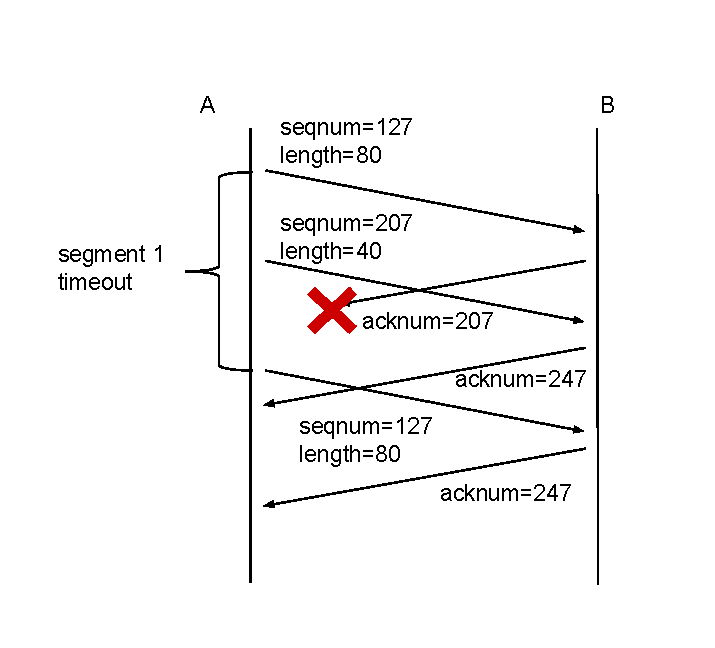
\includegraphics[width=\textwidth]{images/p27.pdf}
    \caption{Coomunication sequence between A and B}
    \label{fig:p27}
\end{figure}
\\


%----------------------------------------------------------------------------------------
%	PROBLEM 31
%----------------------------------------------------------------------------------------

\section*{Problem 31}
After the first measurement:
\begin{align*} 
\begin{split}
EstimatedRTT &= (1-\alpha)*EstimatedRTT + \alpha * SampleRTT \\
&= (1-0.125)*100 + 0.125 * 106 \\
&= 100.75 \quad ms
\end{split}					
\end{align*}
\begin{align*} 
\begin{split}
DevRTT &= (1-\beta)*DevRTT + \beta * | SampleRTT - EstimatedRTT | \\
&= (1-0.25)*5 + 0.25 * | 106 - 100.75 | \\
&= 5.0625 \quad ms
\end{split}					
\end{align*}
\begin{align*} 
\begin{split}
TimeoutInterval &= EstimatedRTT + 4*DevRTT \\
&= 100.75 + 4*5.0625 \\
&= 121 \quad ms
\end{split}					
\end{align*}
After the second measurement:
\begin{align*} 
\begin{split}
EstimatedRTT &= (1-\alpha)*EstimatedRTT + \alpha * SampleRTT \\
&= (1-0.125)*100.75 + 0.125 * 120 \\
&= 103.16 \quad ms
\end{split}					
\end{align*}
\begin{align*} 
\begin{split}
DevRTT &= (1-\beta)*DevRTT + \beta * | SampleRTT - EstimatedRTT | \\
&= (1-0.25)*5.0625 + 0.25 * | 120 - 103.16 | \\
&= 8 \quad ms
\end{split}					
\end{align*}
\begin{align*} 
\begin{split}
TimeoutInterval &= EstimatedRTT + 4*DevRTT \\
&= 103.16 + 4*8 \\
&= 135.16 \quad ms
\end{split}					
\end{align*}
After the third measurement:
\begin{align*} 
\begin{split}
EstimatedRTT &= (1-\alpha)*EstimatedRTT + \alpha * SampleRTT \\
&= (1-0.125)*103.16 + 0.125 * 140 \\
&= 107.765 \quad ms
\end{split}					
\end{align*}
\begin{align*} 
\begin{split}
DevRTT &= (1-\beta)*DevRTT + \beta * | SampleRTT - EstimatedRTT | \\
&= (1-0.25)*8 + 0.25 * | 140 - 107.765 | \\
&= 14.06 \quad ms
\end{split}					
\end{align*}
\begin{align*} 
\begin{split}
TimeoutInterval &= EstimatedRTT + 4*DevRTT \\
&= 107.765 + 4*14.06 \\
&= 164.005 \quad ms
\end{split}					
\end{align*}
After the fourth measurement:
\begin{align*} 
\begin{split}
EstimatedRTT &= (1-\alpha)*EstimatedRTT + \alpha * SampleRTT \\
&= (1-0.125)*107.765 + 0.125 * 90 \\
&= 105.54 \quad ms
\end{split}					
\end{align*}
\begin{align*} 
\begin{split}
DevRTT &= (1-\beta)*DevRTT + \beta * | SampleRTT - EstimatedRTT | \\
&= (1-0.25)*14.06 + 0.25 * | 90 - 105.54 | \\
&= 14.43 \quad ms
\end{split}					
\end{align*}
\begin{align*} 
\begin{split}
TimeoutInterval &= EstimatedRTT + 4*DevRTT \\
&= 105.54 + 4*14.43 \\
&= 163.26 \quad ms
\end{split}					
\end{align*}
After the fifth measurement:
\begin{align*} 
\begin{split}
EstimatedRTT &= (1-\alpha)*EstimatedRTT + \alpha * SampleRTT \\
&= (1-0.125)*105.54 + 0.125 * 115 \\
&= 106.72 \quad ms
\end{split}					
\end{align*}
\begin{align*} 
\begin{split}
DevRTT &= (1-\beta)*DevRTT + \beta * | SampleRTT - EstimatedRTT | \\
&= (1-0.25)*14.43 + 0.25 * | 115 - 106.72 | \\
&= 12.8925 \quad ms
\end{split}					
\end{align*}
\begin{align*} 
\begin{split}
TimeoutInterval &= EstimatedRTT + 4*DevRTT \\
&= 106.72 + 4*12.8925 \\
&= 158.29 \quad ms
\end{split}					
\end{align*}
\\


%----------------------------------------------------------------------------------------
%	PROBLEM 38
%----------------------------------------------------------------------------------------
\section*{Problem 38}
Yes. In the slow start phase, the sending rate is growing exponentially. When congestion occurs,
the sender is sending segments twice more than in previous RTT. This implies, by doubling the sending
rate, sender hits the link limit. So setting ssthresh = cwnd/2 is a proper choice because it gives us
the approximate uncongested sending rate. And the sending rate when congestion occurs should be
roughly cwnd/RTT.



%----------------------------------------------------------------------------------------
%	PROBLEM 40
%----------------------------------------------------------------------------------------

\section*{Problem 40}
(a).
TCP slow start is operating in [1, 6] and [23, 26]. These two segments of curve looks exponential. \\
(b).
Congestion avoidance is operating in [6, 16] and [17, 22]. These two segments show linearity. \\
(c).
It is detected by a triple duplicate ACK. Because the cwnd would have dropped to 1 if timeout occurs. \\
(d).
It is detected by a timeout because cwnd has dropped to 1. \\
(e).
Initial value is 32 because it enters congestion avoidance after $cwnd \geq 32$. \\
(f).
ssthresh is 21 since it should be set to half of cwnd when a triple duplicate ACK occurs. \\
(g).
ssthresh is 14 because when timeout occurs, it will be set to half of the cwnd, which is 28 at round 22. \\
(h).
In the slow start phase, segments sent in each round are 1, 2, 4, 8, 16, 32. So by the end of round 6, 63 segments are sent. And then it goes into congestion avoidance, where $cwnd=32$. So another 32 segments are sent in round 7. That is 95 segments in total. So segmetn 70 is sent in round 7. \\
(i).
After round 26, TCP enters fast recovery mode. It sets the ssthresh to cwnd/2, which is 4. And the new cwnd=ssthresh+3=7. \\
(j).
At round 16, ssthresh is set to cwnd/2=21. And cwnd is set to 1. Then TCP goes to slow start again. Thus, at round 19, the cwnd=4. \\
(k).
A timeout at round 22 would not affect previous rounds. So the total segments sent should be 24+25+26+27+28+29=159. \\


%----------------------------------------------------------------------------------------
%	PROBLEM 45
%----------------------------------------------------------------------------------------

\section*{Problem 45}
\textbf{(a).}
Since there is only one packet lost, and the total number of packets sent is:
\begin{align*} 
\begin{split}
\sum_{0}^{W/2} W/2 + n &= (W/2+1)*W/2+(W/2+1)*W/4 \\
&= \frac{3}{8}*W^2+\frac{3}{4}*W
\end{split}					
\end{align*}
So the loss rate is:
\begin{align*} 
\begin{split}
L &= \frac{1}{\frac{3}{8}*W^2+\frac{3}{4}*W}
\end{split}					
\end{align*}

\textbf{(b).}
Assume all packets are of size MSS. For W that is large enough, L becomes $L=\frac{8}{3*W^2}$.
Solve for W, there is $W=\sqrt{\frac{8}{3L}}$. Then apply to the macroscopic throughput equation:
\begin{align*} 
\begin{split}
\Gamma &= \frac{0.75*W}{RTT} \\
&= 0.75 * \frac{\sqrt{\frac{8}{3L}}}{RTT} \\
&= \frac{1.22}{RTT*\sqrt{L}}
\end{split}					
\end{align*}
And this is in terms of packets, transform it to bits per second, we have:
\begin{align*} 
\begin{split}
\Gamma = \frac{1.22*MSS}{RTT*\sqrt{L}}
\end{split}					
\end{align*}
\\


%----------------------------------------------------------------------------------------
%	PROBLEM 46
%----------------------------------------------------------------------------------------

\section*{Problem 46}
\textbf{(a).}
Since the sending rate is limited by the link capacity, there is:
\begin{align*} 
\begin{split}
10 Mbps &= \frac{W*MSS*8}{RTT} \\
&= \frac{W*1500*8}{0.15}
\end{split}					
\end{align*}
Solve for W, we get $W=125$ segments. \\

\textbf{(b).}
The average window size is:
\begin{align*} 
\begin{split}
W_{avg} &= 0.75*W \\
&= 0.75* 125 = 93.75 = 94\ MSS
\end{split}					
\end{align*}
The average throughput is:
\begin{align*} 
\begin{split}
\Gamma &= \frac{0.75*W}{RTT} \\
&= \frac{W_{avg}*MSS*8}{RTT} \\
&= \frac{94*1500*8}{0.15} \\
&= 7520000 = 7.52 \ Mbps
\end{split}					
\end{align*}

\textbf{(c).}
Since the connection is assumed to be always in congestion avoidance, the window is growing in linear.
After a packet loss, the window size will be reduced to half of the maximum window size.
It needs $W-W/2=W/2$ rounds of RTT to reach maximum again. That is $W/2*RTT=125/2*0.15=9.375 \ ms$
\\


\end{document}
